\lecture{2}{9/14--9/17}{}

\section{Separable Differential Equations}\label{sec:separable}

\source{Boyce §2.2}

The direct-integration idea of \autoref{thm:linear-const} applies to a much larger class
than the linear equations --- including many nonlinear ones.

\begin{notation}
	In this section we use \(x\) rather than \(t\) for the independent variable, both
	because different letters are frequently used and because \(t\) will be reserved for
	another purpose (see \autoref{note:parameter} below).
\end{notation}

Starting from the general first-order equation \(\dfrac{\dd y}{\dd x} = f(x,y)\), rewrite
it as
\begin{equation}\label{eq:MN}
	M(x,y) + N(x,y) \frac{\dd y}{\dd x} = 0.
\end{equation}
This is always possible --- take \(M = -f\) and \(N = 1\) --- but there may be other ways.

\begin{definition}[Separable equation]
	If in~\eqref{eq:MN} \(M\) is a function of \(x\) only and \(N\) is a function of \(y\)
	only, i.e.
	\begin{equation}\label{eq:sep}
		M(x) + N(y) \frac{\dd y}{\dd x} = 0,
	\end{equation}
	then the equation is called \vocab{separable}: writing it in the \vocab{differential
		form}
	\begin{equation}\label{eq:sep-diff}
		M(x) \dd x + N(y) \dd y = 0
	\end{equation}
	the terms involving each variable may be placed on opposite sides.
\end{definition}

\begin{remark}
	The differential form~\eqref{eq:sep-diff} is more symmetric and tends to suppress the
	distinction between the independent and dependent variables.
\end{remark}

\subsection{Examples}

\begin{eg}
	Show that \(\dfrac{\dd y}{\dd x} = \dfrac{x^2}{1 - y^2}\) is separable and find an
	equation for its integral curves.
\end{eg}

\begin{proof}[Solution]
	Write it as \(-x^2 + (1 - y^2) \dfrac{\dd y}{\dd x} = 0\), which has the
	form~\eqref{eq:sep}. Recall the chain rule: if \(y\) is a function of \(x\), then
	\[
		\frac{\dd}{\dd x} F(y) = \frac{\dd}{\dd y}F(y) \cdot \frac{\dd y}{\dd x}
		= F'(y) \frac{\dd y}{\dd x}.
	\]
	Taking \(F(y) = y - y^3/3\) gives \(F'(y) = 1 - y^2\), so the second term is
	\(\dfrac{\dd}{\dd x}\left( y - \frac{y^3}{3}\right)\); the first term is
	\(\dfrac{\dd}{\dd x}\left( -\frac{x^3}{3} \right)\). Hence the equation reads
	\[
		\frac{\dd}{\dd x}\left( -\frac{x^3}{3} + y - \frac{y^3}{3} \right) = 0,
	\]
	and integrating (and multiplying by \(3\)),
	\[
		-x^3 + 3y - y^3 = c.
	\]
	Any differentiable \(y = \varphi(x)\) satisfying this is a solution. The integral
	curve through a given point \((x_0, y_0)\) is found by substituting to determine
	\(c\).
\end{proof}

The same argument works in general.

\begin{theorem}[Solution of a separable equation]\label{thm:sep}
	Let \(H_1, H_2\) be any antiderivatives of \(M, N\), so that \(H_1' = M\) and
	\(H_2' = N\). Then every differentiable \(y = \varphi(x)\) satisfying
	\begin{equation}\label{eq:sep-implicit}
		H_1(x) + H_2(y) = c
	\end{equation}
	is a solution of~\eqref{eq:sep}. Moreover, the solution of the initial value problem
	\(M(x) + N(y) y' = 0\), \(y(x_0) = y_0\) is given implicitly by
	\begin{equation}\label{eq:sep-ivp}
		\int_{x_0}^{x} M(s) \dd s + \int_{y_0}^{y} N(s) \dd s = 0.
	\end{equation}
\end{theorem}

\begin{proof}
	Equation~\eqref{eq:sep} becomes \(H_1'(x) + H_2'(y) \dfrac{\dd y}{\dd x} = 0\).
	Regarding \(y\) as a function of \(x\), the chain rule gives
	\[
		H_2'(y) \frac{\dd y}{\dd x}
		= \frac{\dd}{\dd y}H_2(y) \cdot \frac{\dd y}{\dd x}
		= \frac{\dd}{\dd x} H_2(y),
	\]
	so the equation is \(\dfrac{\dd}{\dd x}\left[ H_1(x) + H_2(y) \right] = 0\).
	Integrating with respect to \(x\) gives~\eqref{eq:sep-implicit}.

	For the initial value problem, setting \(x = x_0\), \(y = y_0\)
	in~\eqref{eq:sep-implicit} gives \(c = H_1(x_0) + H_2(y_0)\). Substituting this back
	and using
	\[
		H_1(x) - H_1(x_0) = \int_{x_0}^{x} M(s)\dd s,
		\qquad
		H_2(y) - H_2(y_0) = \int_{y_0}^{y} N(s)\dd s
	\]
	gives~\eqref{eq:sep-ivp}.
\end{proof}

\begin{remark}
	Equation~\eqref{eq:sep-implicit} defines the solution \emph{implicitly} rather than
	explicitly. In practice one obtains it from~\eqref{eq:sep-diff} by integrating the
	first term with respect to \(x\) and the second with respect to \(y\) --- the
	justification is exactly the argument above. To get an explicit formula one must then
	solve for \(y\), which is often impossible analytically.
\end{remark}

\begin{eg}\label{eg:explicit-quadratic}
	Solve \(\dfrac{\dd y}{\dd x} = \dfrac{3x^2 + 4x + 2}{2(y-1)}\), \(y(0) = -1\), and
	determine the interval on which the solution exists.
\end{eg}

\begin{proof}[Solution]
	In differential form, \(2(y-1)\dd y = (3x^2 + 4x + 2)\dd x\). Integrating each side,
	\[
		y^2 - 2y = x^3 + 2x^2 + 2x + c.
	\]
	Substituting \(x = 0\), \(y = -1\) gives \(c = 3\), so implicitly
	\[
		y^2 - 2y = x^3 + 2x^2 + 2x + 3.
	\]
	This is quadratic in \(y\), so we can solve explicitly:
	\[
		y = 1 \pm \sqrt{x^3 + 2x^2 + 2x + 4}.
	\]
	Only \emph{one} of these two branches satisfies the initial condition --- the minus
	sign --- so
	\[
		y = \varphi(x) = 1 - \sqrt{x^3 + 2x^2 + 2x + 4}.
	\]
	(The plus sign would give the solution with \(y(0) = 3\) instead.) The solution is
	valid where the radicand is positive; its only real zero is \(x = -2\), so the
	interval of validity is \(x > -2\). Note that the boundary of that interval is the
	point \((-2, 1)\), at which the tangent line is \emph{vertical}.
\end{proof}

\begin{eg}
	Solve \(\dfrac{\dd y}{\dd x} = \dfrac{4x - x^3}{4 + y^3}\), find the solution through
	\((0,1)\), and determine its interval of validity.
\end{eg}

\begin{proof}[Solution]
	Rewriting as \((4 + y^3)\dd y = (4x - x^3)\dd x\), integrating, multiplying by \(4\)
	and rearranging,
	\[
		y^4 + 16y + x^4 - 8x^2 = c.
	\]
	Substituting \(x = 0\), \(y = 1\) gives \(c = 17\), so the solution is given
	implicitly by
	\[
		y^4 + 16y + x^4 - 8x^2 = 17.
	\]
	Here we \emph{cannot} solve explicitly for \(y\). The interval of validity extends on
	either side of the initial point as long as the function remains differentiable, i.e.\
	until the tangent line becomes vertical. From the differential equation, this happens
	where \(4 + y^3 = 0\), i.e.\ \(y = (-4)^{1/3} \approx -1.5874\); the corresponding
	values are \(x \approx \pm 3.3488\).
\end{proof}

\begin{note}[Constant solutions]
	If \(f(x, y_0) = 0\) for some value \(y_0\) and \emph{all} \(x\), then the constant
	function \(y \equiv y_0\) is a solution of \(\dd y/\dd x = f(x,y)\). Such solutions
	are usually easy to spot. For example
	\[
		\frac{\dd y}{\dd x} = \frac{(y-3)\cos x}{1 + 2y^2}
	\]
	has the constant solution \(y \equiv 3\); the other solutions are found by separating
	variables.
\end{note}

\begin{note}[Introducing a parameter]\label{note:parameter}
	It sometimes helps to regard \emph{both} \(x\) and \(y\) as functions of a third
	variable \(t\), so that
	\[
		\frac{\dd y}{\dd x} = \frac{\dd y/\dd t}{\dd x/\dd t}.
	\]
	Comparing numerators and denominators, the equation
	\(\dfrac{\dd y}{\dd x} = \dfrac{F(x,y)}{G(x,y)}\) becomes the system
	\[
		\frac{\dd x}{\dd t} = G(x,y), \qquad \frac{\dd y}{\dd t} = F(x,y).
	\]
	Replacing one equation by a pair may seem like a step backwards, but the system is
	often more amenable to investigation.
\end{note}

\begin{note}[On the phrase ``solve the equation'']
	Being able to solve explicitly for \(y\), as in \autoref{eg:explicit-quadratic}, is
	exceptional; often it is better to leave the solution in implicit form. Accordingly,
	``solve the following differential equation'' means: find the solution explicitly if
	convenient, and otherwise find an equation defining it implicitly.
\end{note}

\subsection{Homogeneous Equations \texorpdfstring{\(y' = g(y/x)\)}{y' = g(y/x)}}

\source{Boyce §2.2, Problem 25 --- promoted to a method here}

Some equations that are \emph{not} separable become separable after a change of the
dependent variable. The most important such family is the following.

\begin{definition}[Homogeneous equation]
	The equation \(\dfrac{\dd y}{\dd x} = f(x,y)\) is called \vocab{homogeneous} if the
	right-hand side depends on \(x\) and \(y\) only through their ratio, i.e.\ if there
	is a function \(g\) of one variable with
	\begin{equation}\label{eq:homog}
		\frac{\dd y}{\dd x} = g\!\left( \frac{y}{x} \right).
	\end{equation}
\end{definition}

\begin{abuse}
	The word ``homogeneous'' has a completely different meaning for linear equations
	(there it means \(g(t) \equiv 0\) in~\eqref{eq:std}, as in Boyce Chapter 3). The two
	notions have nothing to do with each other; only the context distinguishes them.
\end{abuse}

\begin{observation}[Why the name, and what it looks like]
	Condition~\eqref{eq:homog} says precisely that \(f\) is invariant under the scaling
	\((x,y) \mapsto (\lambda x, \lambda y)\):
	\[
		f(\lambda x, \lambda y) = f(x, y) \quad \text{for all } \lambda \neq 0.
	\]
	Geometrically, \textbf{the direction field is constant along every ray through the
		origin}. So the whole picture is determined by what happens on a single circle around
	the origin, and it should not be a surprise that one variable can be eliminated.
\end{observation}

\begin{figure}[H]
	\centering
	\begin{tikzpicture}
		\begin{axis}[
				width=0.55\textwidth, height=5.5cm,
				xlabel={$x$}, ylabel={$y$},
				xmin=-3, xmax=3, ymin=-3, ymax=3,
				axis lines=middle,
				xtick={-2,2}, ytick={-2,2},
				every axis x label/.style={at={(ticklabel* cs:1.0)},anchor=west},
				every axis y label/.style={at={(ticklabel* cs:1.0)},anchor=south},
			]
			\foreach \X in {-2.75,-2.25,...,2.75}{
					\foreach \Y in {-2.65,-2.15,...,2.85}{
							\pgfmathsetmacro{\Sl}{(\X+\Y)/(\X-\Y)}%
							\slopemark{gray!75}{\X}{\Y}{\Sl}{1.467}{0.917}
						}
				}
			\addplot[very thick, RawSienna, dashed, domain=-3:3, samples=2]{0.5*x};
			\addplot[very thick, MidnightBlue, dashed, domain=-3:3, samples=2]{-1.5*x};
		\end{axis}
	\end{tikzpicture}
	\caption{Direction field of the homogeneous equation
		\(y' = (x+y)/(x-y)\). Along each dashed ray \(y = vx\) the slope is the same
		constant \(g(v)\) --- this is what ``homogeneous'' means.}
\end{figure}

\begin{theorem}[Reduction to a separable equation]\label{thm:homog}
	Substituting
	\[
		v = \frac{y}{x}, \qquad\text{i.e.}\qquad y = v x,
	\]
	turns the homogeneous equation~\eqref{eq:homog} into the separable equation
	\begin{equation}\label{eq:homog-sep}
		x \frac{\dd v}{\dd x} = g(v) - v.
	\end{equation}
\end{theorem}

\begin{proof}
	Regard \(v\) as a new unknown function of \(x\). By the product rule,
	\[
		\frac{\dd y}{\dd x} = \frac{\dd}{\dd x}(v x) = v + x \frac{\dd v}{\dd x},
	\]
	while the right-hand side of~\eqref{eq:homog} is \(g(v)\). Equating the two and
	rearranging gives~\eqref{eq:homog-sep}, in which the variables separate as
	\[
		\frac{\dd v}{g(v) - v} = \frac{\dd x}{x}
		\qquad \text{whenever } g(v) \neq v. \qedhere
	\]
\end{proof}

\begin{remark}[Equilibria of the reduced equation]
	The roots of \(g(v) = v\) --- excluded above --- are exactly the equilibrium solutions
	of~\eqref{eq:homog-sep}. Each root \(v_0\) gives a \emph{straight-line} solution
	\(y = v_0 x\) of the original equation. These are worth finding first; they are
	the rays along which the direction field points radially.
\end{remark}

\begin{eg}
	Solve \(\dfrac{\dd y}{\dd x} = \dfrac{x^2 + xy + y^2}{x^2}\).
\end{eg}

\begin{proof}[Solution]
	Dividing numerator and denominator by \(x^2\),
	\[
		\frac{\dd y}{\dd x} = 1 + \frac{y}{x} + \left( \frac{y}{x} \right)^{2}
		= g\!\left( \frac{y}{x} \right), \qquad g(v) = 1 + v + v^2,
	\]
	so the equation is homogeneous. Note \(g(v) - v = 1 + v^2\), which never vanishes, so
	there are no straight-line solutions. By \autoref{thm:homog},
	\[
		x \frac{\dd v}{\dd x} = 1 + v^{2}
		\implies \frac{\dd v}{1 + v^{2}} = \frac{\dd x}{x}
		\implies \arctan v = \ln\abs{x} + c.
	\]
	Hence \(v = \tan\left( \ln\abs{x} + c \right)\), and restoring \(y = vx\),
	\[
		y = x \tan\left( \ln\abs{x} + c \right).
	\]
\end{proof}

\begin{eg}
	Solve \(\dfrac{\dd y}{\dd x} = \dfrac{y^2 + 2xy}{x^2}\).
\end{eg}

\begin{proof}[Solution]
	Here \(g(v) = v^2 + 2v\), so \(g(v) - v = v^2 + v = v(v+1)\). The roots \(v = 0\) and
	\(v = -1\) give the straight-line solutions \(y = 0\) and \(y = -x\). Otherwise,
	\[
		\frac{\dd v}{v(v+1)} = \frac{\dd x}{x}
		\implies \int \left( \frac{1}{v} - \frac{1}{v+1} \right) \dd v = \ln\abs{x} + c,
	\]
	using partial fractions. Thus \(\ln\left| \dfrac{v}{v+1} \right| = \ln\abs{x} + c\),
	i.e.\ \(\dfrac{v}{v+1} = Kx\) for a constant \(K\). Substituting \(v = y/x\) and
	solving,
	\[
		\frac{y}{y + x} = Kx
		\implies y = \frac{K x^{2}}{1 - Kx}.
	\]
\end{proof}

\begin{moral}
	The pattern is worth remembering, because it recurs: \emph{find a change of variable
		that turns a problem you cannot do into one you can}. Separable equations are the
	base case; ``homogeneous'' is the first of many families that reduce to it.
\end{moral}

\section{Modeling with First-Order Differential Equations}

\source{Boyce §2.3}

\begin{moral}
	Regardless of the field of application, three steps are always present in mathematical
	modelling.
	\begin{description}
		\item[Step 1: Construction of the model.] Translate the physical situation into
			mathematical terms, stating clearly the physical principle(s) believed to govern
			the process. Each such principle involves a \emph{rate of change} and hence leads
			to a differential equation.
		\item[Step 2: Analysis of the model.] Solve the resulting equation(s) or, failing
			that, find out as much as possible about the properties of the solution. Further
			approximations may be needed here (linearizing a nonlinear equation, replacing a
			slowly varying coefficient by a constant) --- but each must be checked against
			the physics.
		\item[Step 3: Comparison with experiment or observation.] Interpret the solution in
			the context in which the problem arose, and check that it is physically
			reasonable. Serious inconsistency with observation means either an error in the
			solution, a model in need of refinement, or observations needing more care.
	\end{description}
\end{moral}

\begin{remark}
	The equations are almost always only an \emph{approximate} description of the actual
	process: bodies moving near the speed of light are not governed by Newton's laws,
	insect populations do not grow indefinitely, heat transfer depends on more than the
	temperature difference. Modelling also often replaces a discrete process by a
	continuous one --- an insect population changes by whole numbers, but if it is large
	it is reasonable to treat it as a continuous variable and even to differentiate it.
\end{remark}

\subsection{Mixing}

\begin{eg}[A salt tank]
	At time \(t = 0\) a tank contains \(Q_0\) lb of salt dissolved in \(100\) gal of
	water. Water containing \(\frac14\) lb of salt per gallon enters at \(r\) gal/min, and
	the well-stirred mixture drains at the same rate. Find \(Q(t)\), the amount of salt at
	time \(t\), and the limiting amount \(Q_L\). If \(r = 3\) and \(Q_0 = 2Q_L\), find the
	time \(T\) after which the salt level is within \(2\%\) of \(Q_L\); and find the flow
	rate needed so that \(T \leq 45\) min.
\end{eg}

\begin{proof}[Solution]
	Salt is neither created nor destroyed, so
	\begin{equation}\label{eq:balance}
		\frac{\dd Q}{\dd t} = \text{rate in} - \text{rate out}.
	\end{equation}
	\begin{itemize}
		\item \textbf{Rate in:} concentration \(\times\) flow rate
		      \(= \frac14 \cdot r = r/4\) lb/min.
		\item \textbf{Rate out:} since inflow and outflow rates are equal, the volume stays
		      at \(100\) gal; since the mixture is well stirred, the concentration is uniform
		      and equal to \(Q(t)/100\) lb/gal. So the rate out is \(rQ(t)/100\) lb/min.
	\end{itemize}
	Hence the IVP is
	\begin{equation}\label{eq:mixing}
		\frac{\dd Q}{\dd t} = \frac{r}{4} - \frac{rQ}{100}, \qquad Q(0) = Q_0.
	\end{equation}
	Setting \(\dd Q/\dd t = 0\) gives \(Q_L = 25\) lb immediately --- as physical
	intuition suggests, since the tank is eventually filled with the incoming mixture of
	concentration \(\frac14\) lb/gal.

	Equation~\eqref{eq:mixing} is linear (and also separable). In standard form,
	\(Q' + \frac{r}{100}Q = \frac{r}{4}\), with integrating factor \(e^{rt/100}\), giving
	the general solution \(Q(t) = 25 + ce^{-rt/100}\). The initial condition gives
	\(c = Q_0 - 25\), so
	\begin{equation}\label{eq:mixing-sol}
		Q(t) = 25 + (Q_0 - 25) e^{-rt/100}
		= \underbrace{25\left( 1 - e^{-rt/100} \right)}_{\text{salt from the inflow}}
		+ \underbrace{Q_0 e^{-rt/100}}_{\text{original salt remaining}}.
	\end{equation}
	Either form shows \(Q(t) \to 25\) as \(t \to \infty\), confirming \(Q_L = 25\), and
	that the approach is faster for larger \(r\).

	Now take \(r = 3\) and \(Q_0 = 2Q_L = 50\), so \(Q(t) = 25 + 25e^{-0.03t}\). Since
	\(2\%\) of \(25\) is \(0.5\), we want \(Q(T) = 25.5\):
	\[
		25e^{-0.03T} = 0.5 \implies T = \frac{\ln 50}{0.03} \approx 130.4 \text{ min}.
	\]
	To achieve \(T = 45\) instead, set \(t = 45\), \(Q_0 = 50\), \(Q = 25.5\)
	in~\eqref{eq:mixing-sol} and solve for \(r\):
	\[
		r = \frac{100}{45}\ln 50 \approx 8.69 \text{ gal/min}.
	\]
\end{proof}

\begin{observation}
	Equation~\eqref{eq:mixing} is another relaxation process (\autoref{cor:relax}), with
	\(Q_{\mathrm{eq}} = 25\) and relaxation time \(\tau = 100/r\) minutes. The tank
	forgets its initial contents on the time scale of one ``tank volume'' of throughput.
\end{observation}

\begin{remark}
	Models of this kind are used for a pollutant in a lake or a drug in an organ of the
	body, not just salt in a tank. In such cases the flow rates may be hard to determine
	or may vary with time, the concentration may be far from uniform, and the inflow and
	outflow rates may differ --- in which case the changing volume of liquid must also be
	tracked.
\end{remark}

\subsection{Seasonal Growth}

In \autoref{sec:relax} the coefficients were constants. Real environments vary with the
seasons, which makes the coefficients \emph{periodic functions of \(t\)} --- and the
techniques of §2.1 and §2.2 handle this at no extra cost.

\begin{eg}[A seasonally varying growth rate]
	A population grows at a rate that varies with the season:
	\begin{equation}\label{eq:seasonal}
		\frac{\dd y}{\dd t} = \left( 0.5 + \sin t \right) \frac{y}{5},
		\qquad y(0) = 1.
	\end{equation}
	Find the doubling time \(\tau\), and compare it with the doubling time obtained by
	replacing the growth rate by its average value \(0.1\).
\end{eg}

\begin{proof}[Solution]
	Equation~\eqref{eq:seasonal} is separable (it is also linear). Separating,
	\[
		\frac{\dd y}{y} = \frac{0.5 + \sin t}{5} \dd t
		\implies \ln y = \frac{0.5 t - \cos t}{5} + C,
	\]
	and \(y(0) = 1\) fixes \(C = 1/5\). Hence
	\begin{equation}\label{eq:seasonal-sol}
		y(t) = \exp\left( 0.1 t + \frac{1 - \cos t}{5} \right)
		= \exp\left( 0.1t + 0.2\left( 1 - \cos t \right) \right).
	\end{equation}
	The doubling time solves \(0.1\tau + 0.2(1 - \cos \tau) = \ln 2\), which has no
	closed-form solution; numerically \(\tau \approx 6.73\). Replacing the growth rate by
	its average \(0.1\) gives instead \(y = e^{0.1t}\) and
	\(\tau_{\text{avg}} = \ln 2 / 0.1 \approx 6.93\).
\end{proof}

\begin{observation}
	Two things are worth noticing.
	\begin{enumerate}[(i)]
		\item Because~\eqref{eq:seasonal-sol} is \(y_0\) times a function of \(t\) alone,
		      the doubling time does \emph{not} depend on the initial population. This is
		      special to the linear growth law; it fails as soon as crowding is modelled.
		\item The seasonal solution is not the averaged solution: the oscillating term
		      \(0.2(1 - \cos t)\) is never negative, so~\eqref{eq:seasonal-sol} runs
		      \emph{ahead} of \(e^{0.1t}\) and doubles sooner. Averaging the coefficients of a
		      differential equation is not the same as averaging its solutions.
	\end{enumerate}
\end{observation}

\begin{figure}[H]
	\centering
	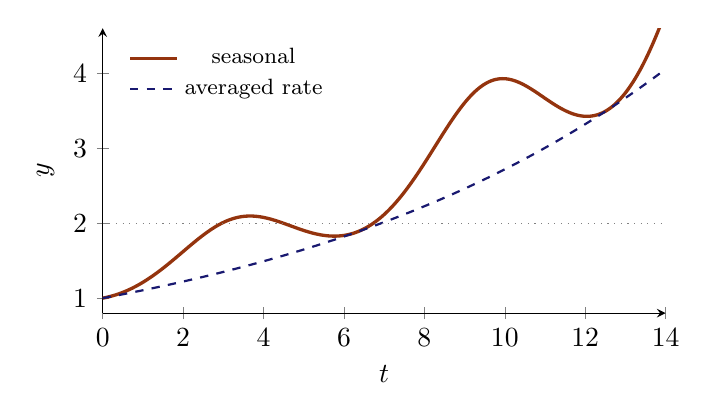
\begin{tikzpicture}
		\begin{axis}[
				width=0.72\textwidth, height=5.2cm,
				xlabel={$t$}, ylabel={$y$},
				xmin=0, xmax=14, ymin=0.8, ymax=4.6,
				axis lines=left, legend pos=north west,
				legend style={draw=none, font=\footnotesize, fill=none},
			]
			\addplot[very thick, RawSienna, domain=0:14, samples=300]
			{exp(0.1*x + 0.2*(1-cos(deg(x))))};
			\addlegendentry{seasonal}
			\addplot[thick, MidnightBlue, dashed, domain=0:14, samples=100]
			{exp(0.1*x)};
			\addlegendentry{averaged rate}
			\addplot[gray, dotted, domain=0:14, samples=2]{2};
		\end{axis}
	\end{tikzpicture}
	\caption{Solution~\eqref{eq:seasonal-sol} against the constant-rate solution
		\(e^{0.1t}\). The seasonal population crosses \(y = 2\) at
		\(\tau \approx 6.73\), slightly before \(\tau_{\text{avg}} \approx 6.93\).}
\end{figure}

The same idea applies when it is the \emph{input} that varies seasonally rather than the
growth rate.

\begin{eg}[Chemicals in a pond]
	A pond initially contains \(10\) million gallons of fresh water. Water containing an
	undesirable chemical flows in at \(5\) million gal/year and the mixture flows out at
	the same rate. The incoming concentration varies periodically:
	\(\gamma(t) = 2 + \sin(2t)\) g/gal. Find the amount of chemical in the pond at any
	time.
\end{eg}

\begin{proof}[Solution]
	The volume stays at \(10^7\) gal. Let \(t\) be measured in years and \(Q(t)\) in
	grams. By the same balance law~\eqref{eq:balance},
	\[
		\text{rate in} = (5 \times 10^6)\left( 2 + \sin(2t) \right) \text{ g/yr},
		\qquad
		\text{rate out} = (5 \times 10^6)\cdot \frac{Q(t)}{10^7} = \frac{Q(t)}{2}
		\text{ g/yr},
	\]
	so
	\[
		\frac{\dd Q}{\dd t} = (5\times 10^6)\left( 2 + \sin (2t) \right)
		- \frac{Q(t)}{2}.
	\]
	To tame the coefficients, set \(q(t) = Q(t)/10^6\) (so \(q\) is measured in
	megagrams, i.e.\ metric tons). Every term then carries a factor \(10^6\), which
	cancels:
	\begin{equation}\label{eq:pond}
		\frac{\dd q}{\dd t} + \frac{1}{2}q = 10 + 5\sin(2t), \qquad q(0) = 0.
	\end{equation}
	This is linear with constant coefficient, so \(\mu(t) = e^{t/2}\), and integrating
	gives the general solution
	\[
		q(t) = 20 - \frac{40}{17}\cos(2t) + \frac{10}{17}\sin(2t) + ce^{-t/2}.
	\]
	The initial condition requires \(c = -300/17\), so
	\begin{equation}\label{eq:pond-sol}
		q(t) = 20 - \frac{40}{17}\cos(2t) + \frac{10}{17}\sin(2t)
		- \frac{300}{17} e^{-t/2}.
	\end{equation}
\end{proof}

\begin{figure}[H]
	\centering
	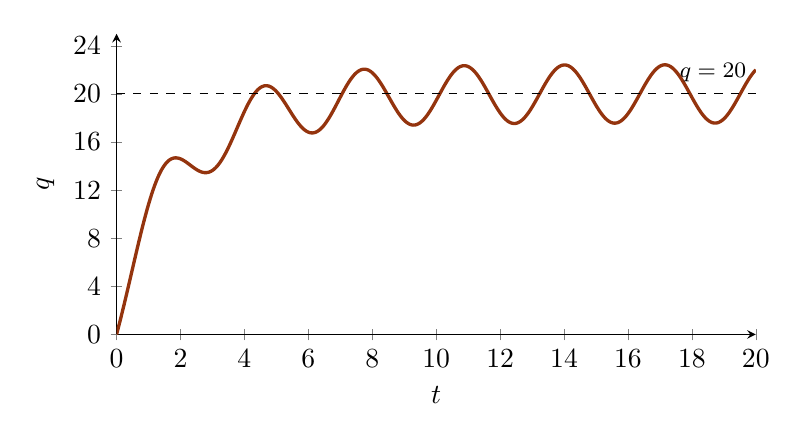
\begin{tikzpicture}
		\begin{axis}[
				width=0.8\textwidth, height=5.4cm,
				xlabel={$t$}, ylabel={$q$},
				xmin=0, xmax=20, ymin=0, ymax=25,
				ytick={0,4,8,12,16,20,24},
				axis lines=left,
			]
			\addplot[very thick, RawSienna, domain=0:20, samples=400]
			{20 - (40/17)*cos(deg(2*x)) + (10/17)*sin(deg(2*x)) - (300/17)*exp(-x/2)};
			\addplot[black, dashed, domain=0:20, samples=2]{20};
			\node[anchor=south east, font=\footnotesize] at (axis cs:20,20.2) {$q=20$};
		\end{axis}
	\end{tikzpicture}
	\caption{Solution~\eqref{eq:pond-sol} of the pond problem
		\(q' + q/2 = 10 + 5\sin(2t)\), \(q(0) = 0\).}
\end{figure}

\begin{observation}
	The exponential term matters for small \(t\) but decays rapidly; thereafter the
	solution oscillates about the constant level \(q = 20\). Were the \(\sin(2t)\) term
	absent from~\eqref{eq:pond}, \(q = 20\) would be exactly the equilibrium solution.
	With it, the system settles not onto a point but onto a \emph{periodic} response
	of the same frequency as the forcing --- the \vocab{steady state} --- while the part
	that remembers the initial condition, the \vocab{transient}, dies out on the
	relaxation time \(\tau = 2\) years.
\end{observation}

\begin{remark}
	This model assumes the water level is controlled entirely by the flows --- no
	evaporation, seepage or rainfall --- that no chemical is absorbed by fish or other
	organisms, and that the concentration is uniform throughout the pond.
\end{remark}

\subsection{Compound Interest}

\begin{eg}[Continuous compounding]
	A sum \(S_0\) is deposited in an account paying interest at annual rate \(r\),
	compounded \emph{continuously}. Find the value \(S(t)\).
\end{eg}

\begin{proof}[Solution]
	The rate of change of the investment equals the rate at which interest accrues, which
	is \(r\) times the current value:
	\[
		\frac{\dd S}{\dd t} = rS, \qquad S(0) = S_0.
	\]
	This equation is both linear and separable, and gives
	\[
		S(t) = S_0 e^{rt};
	\]
	a continuously compounded account grows exponentially.
\end{proof}

If deposits or withdrawals also occur at a constant rate \(k\) (positive for deposits,
negative for withdrawals), the model becomes
\begin{equation}\label{eq:interest-k}
	\frac{\dd S}{\dd t} - rS = k,
\end{equation}
which is linear with integrating factor \(e^{-rt}\), so \(S(t) = ce^{rt} - k/r\). The
initial condition forces \(c = S_0 + k/r\), whence
\begin{equation}\label{eq:interest-sol}
	S(t) = \underbrace{S_0 e^{rt}}_{\text{return on the initial amount}}
	+ \underbrace{\frac{k}{r}\left( e^{rt} - 1 \right)}_{\text{due to deposits/withdrawals}}.
\end{equation}

\begin{eg}[A retirement account]
	Someone opens a retirement account at age \(25\) and invests \(\$2000\) per year
	continuously thereafter, at a rate of return of \(8\%\). What is the balance at age
	\(65\)?
\end{eg}

\begin{proof}[Solution]
	Here \(S_0 = 0\), \(r = 0.08\), \(k = 2000\), and we want \(S(40)\).
	By~\eqref{eq:interest-sol},
	\[
		S(40) = \frac{2000}{0.08}\left( e^{3.2} - 1 \right)
		= 25{,}000 \left( e^{3.2} - 1 \right) \approx \$588{,}313.
	\]
	The total amount invested is only \(\$80{,}000\); the remaining \(\$508{,}313\) is
	accumulated return. The result is quite sensitive to \(r\): with \(r = 0.075\) one
	gets \(\$508{,}948\), and with \(r = 0.085\), \(\$681{,}508\).
\end{proof}

\begin{remark}[Continuous versus discrete compounding]
	If interest is compounded \(m\) times per year, then
	\[
		S(t) = S_0 \left( 1 + \frac{r}{m} \right)^{mt},
	\]
	and the connection with the continuous model is the familiar limit
	\[
		\lim_{m \to \infty} S_0 \left( 1 + \frac{r}{m} \right)^{mt} = S_0 e^{rt}.
	\]
	In practice the frequency of compounding matters little: at \(r = 8\%\), over ten
	years the difference between quarterly and continuous compounding is about
	\(\$17.50\) per \(\$1000\) invested, i.e.\ under \(\$2\) per year. (The annual yield
	is \(8.24\%\) for quarterly and \(8.33\%\) for daily or continuous compounding.)
\end{remark}

\begin{notation}
	Since the same model applies to investments accruing dividends and capital gains as
	well as interest, we refer to \(r\) as the \vocab{rate of return}.
\end{notation}

\subsection{Escape Velocity}

\begin{eg}[Escape velocity]
	A body of constant mass \(m\) is projected away from the earth perpendicular to its
	surface with initial velocity \(v_0\). Ignoring air resistance but taking into account
	the variation of gravity with distance, find the velocity during the ensuing motion,
	the initial velocity needed to reach a maximum altitude \(A_{\max}\), and the least
	initial velocity for which the body never returns --- the \vocab{escape velocity}.
\end{eg}

\begin{proof}[Solution]
	Let the positive \(x\)-axis point away from the centre of the earth along the line of
	motion, with \(x = 0\) on the surface and \(R\) the radius of the earth. The
	gravitational force (the body's weight) is inversely proportional to the square of the
	distance from the earth's centre:
	\[
		w(x) = -\frac{k}{(x+R)^2}.
	\]
	At the surface \(w(0) = -mg\), so \(k = mgR^2\) and \(w(x) = -mgR^2/(R+x)^2\). Since
	no other force acts, Newton's second law gives
	\begin{equation}\label{eq:escape-t}
		m \frac{\dd v}{\dd t} = -\frac{mgR^2}{(R+x)^2}, \qquad v(0) = v_0.
	\end{equation}
	Unfortunately~\eqref{eq:escape-t} involves \emph{three} variables \(t\), \(x\) and
	\(v\). The trick is to eliminate \(t\) by taking \(x\) as the independent variable;
	by the chain rule,
	\[
		\frac{\dd v}{\dd t} = \frac{\dd v}{\dd x}\frac{\dd x}{\dd t}
		= v \frac{\dd v}{\dd x},
	\]
	so that
	\begin{equation}\label{eq:escape-x}
		v \frac{\dd v}{\dd x} = -\frac{gR^2}{(R+x)^2}.
	\end{equation}
	Equation~\eqref{eq:escape-x} is separable (but not linear); separating and
	integrating,
	\[
		\frac{v^2}{2} = \frac{gR^2}{R+x} + c.
	\]
	Since \(x = 0\) when \(t = 0\), the initial condition becomes \(v = v_0\) at
	\(x = 0\), giving \(c = v_0^2/2 - gR\) and
	\begin{equation}\label{eq:escape-v}
		v = \pm\sqrt{v_0^2 - 2gR + \frac{2gR^2}{R+x}},
	\end{equation}
	with the plus sign while the body rises and the minus sign while it falls back.

	Note that~\eqref{eq:escape-v} gives velocity as a function of \emph{altitude}, not of
	time. Setting \(v = 0\) and \(x = A_{\max}\) and solving,
	\[
		A_{\max} = \frac{v_0^2 R}{2gR - v_0^2},
		\qquad\text{equivalently}\qquad
		v_0 = \sqrt{2gR\,\frac{A_{\max}}{R + A_{\max}}}.
	\]
	Letting \(A_{\max} \to \infty\) gives the escape velocity
	\begin{equation}\label{eq:ve}
		v_e = \sqrt{2gR} \approx \SI{11.1}{\kilo\metre\per\second}
		\approx 6.9\ \text{mi/s}.
	\end{equation}
\end{proof}

\begin{observation}
	The trick used here --- trading the independent variable \(t\) for the state variable
	\(x\) --- is worth remembering. It works whenever the force depends on position but
	not explicitly on time, and it is the differential-equations shadow of conservation of
	energy: multiplying \(m\ddot{x} = F(x)\) by \(\dot x\) and integrating gives
	\(\frac12 m v^2 - \int F = \text{const}\), which is what
	equation~\eqref{eq:escape-v} says.
\end{observation}

\begin{remark}
	This calculation neglects air resistance, so the true escape velocity is somewhat
	higher. On the other hand, launching from high altitude reduces both gravitational and
	frictional forces (air resistance in particular falls off rapidly with altitude). Note
	too that it is impractical to impart such a large velocity instantaneously; real space
	vehicles accelerate over a period of minutes.
\end{remark}
